\let\negmedspace\undefined
\let\negthickspace\undefined
\documentclass[journal,12pt,twocolumn]{IEEEtran}
\usepackage{cite}
\usepackage{amsmath,amssymb,amsfonts,amsthm}
\usepackage{algorithmic}
\usepackage{graphicx}
\usepackage{textcomp}
\usepackage{xcolor}
\usepackage{txfonts}
\usepackage{listings}
\usepackage{enumitem}
\usepackage{mathtools}
\usepackage{gensymb}
\usepackage[breaklinks=true]{hyperref}
\usepackage{tkz-euclide} % loads  TikZ and tkz-base
\usepackage{listings}
\usepackage{gvv}
\usepackage{circuitikz}
\newtheorem{theorem}{Theorem}[section]
\newtheorem{problem}{Problem}
\newtheorem{proposition}{Proposition}[section]
\newtheorem{lemma}{Lemma}[section]
\newtheorem{corollary}[theorem]{Corollary}
\newtheorem{example}{Example}[section]
\newtheorem{definition}[problem]{Definition}
%\newtheorem{thm}{Theorem}[section] 
%\newtheorem{defn}[thm]{Definition}
%\newtheorem{algorithm}{Algorithm}[section]
%\newtheorem{cor}{Corollary}
\newcommand{\BEQA}{\begin{eqnarray}}
\newcommand{\EEQA}{\end{eqnarray}}
\newcommand{\define}{\stackrel{\triangle}{=}}
\theoremstyle{remark}
\newtheorem{rem}{Remark}

%\bibliographystyle{ieeetr}
\begin{document}
%

\bibliographystyle{IEEEtran}


\vspace{3cm}

\title{
%  \logo{
GATE AE-62 (2022)

\large{EE:1205 \brak{Signals Systems}}

Indian Institute of Technology, Hyderabad
%  }
}
\author{Md Ayaan Ashraf

EE23BTECH11041
}  
\maketitle
\newpage
\bigskip
\renewcommand{\thefigure}{\arabic{figure}}
\renewcommand{\thetable}{\arabic{table}}
%\renewcommand{\theequation}{\theenumi}
\section*{\textit{\textbf{Question}}}
A damper with damping coefficient, $c$, is attached to a mass of $5$ \text{kg} and spring of stiffness  $5$ \text{kN/m} as shown in figure. The system undergoes under-damped oscillations.
If the ratio of the $3^{rd}$ amplitude to the $4^{th}$ amplitude of oscillations is ${1.5}$, the value of $c$ is ?
\begin{figure}[ht]
    \centering
    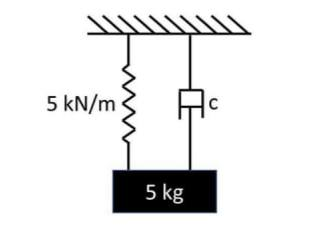
\includegraphics[width=\columnwidth]{figs/fig1.png}
\end{figure}

\hfill {(GATE AE-62 (2022))}
\section*{\textit{\textbf{Solution:}}}

\begin{table}[ht]
  \begin{tabular}{|c||c||c|}
    \hline
    \textbf{Parameter} & \textbf{Value} & \textbf{Description} \\
    \hline
    $c$ & $? $ & Damping Coefficient \\
    \hline
    $k$ & $5$ \text{kN/m} & Stiffness \\
    \hline
    $r$ & $1.5$ & Ratio of $3^{rd}$ amplitude to $4^{th}$ \\&& amplitude of oscillations \\
    \hline
  \end{tabular}
  \vspace{2mm}
  \caption{Parameter Table (GATE AE-62)}
\end{table}


    \begin{figure}[h]
        \centering
        
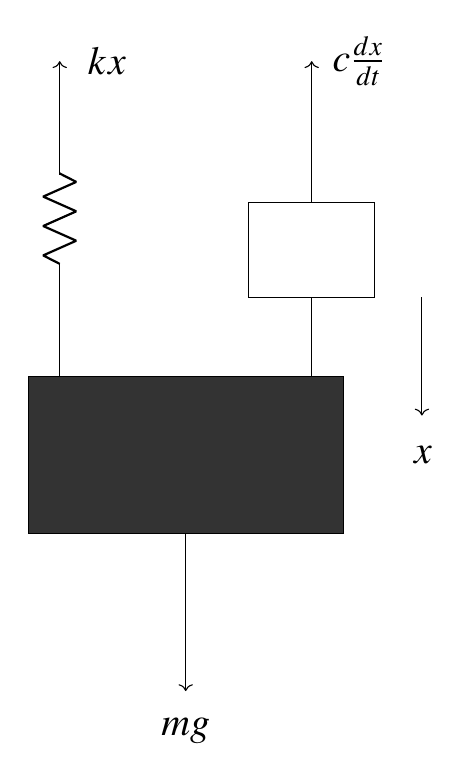
\begin{tikzpicture}[scale=1]
\draw (0,0) rectangle (4,2);
  \filldraw[fill=black!80] (0,0) rectangle (4,2);
\draw (0.4,2) -- (0.4,3);
% \draw[decorate,decoration={coil,amplitude=6pt,segment length=7pt}] (0.4,3) -- (0.4,5);
\draw (0.4,3) to [R] (0.4,5);
\draw [->](0.4,5)--(0.4,6);
\draw (3.6,2) -- (3.6,3);
\draw (2.8,3) rectangle (4.4,4.2);
\draw [->](3.6,4.2)--(3.6,6);

 \node at (4.2,6) {\Large$c\frac{dx}{dt}$};
 \node at (1,6) {\Large$kx$}; 
 \draw[->] (5,3)  -- (5,1.5);
 \node at (5,1) {\Large $x$};

 \draw[->](2,0) -- (2,-2);
 \node at (2,-2.5) {\Large$mg$};
\end{tikzpicture}


        \label{fig:Fig-1}
    \end{figure}

    Now, as the oscillation begins, from the \figref{fig:Fig-1} we write net force on the mass as,
    \begin{align}
        &F=F_{1}+F_{2}+mgu(t) \label{eq:3}\\
        \implies &m\frac{d^2x(t)}{dt^2}=-kx(t)-c\frac{dx(t)}{dt}+mgu(t) \label{eq:4}\\
        \implies &\frac{d^2x(t)}{dt^2}+\brak{\frac{c}{m}}\frac{dx(t)}{dt}+\brak{\frac{k}{m}}x(t)=gu(t) \label{eq:5}
    \end{align}

    Now, taking the Laplace transform on both sides,
    \begin{align}
        &s^2X(s)+\frac{c}{m}sX(s)+\frac{k}{m}X(s)=\frac{g}{s} \label{eq:6}\\
        \implies &X(s)=\frac{g}{s\brak{(s^2+\frac{c}{m}s+\frac{k}{m}}} \label{eq:7}\\
        \implies &X(s)=\frac{g}{s(s-s_1)(s-s_2)} \label{eq:8}
    \end{align}
    Where
    \begin{align}
        &s_1=-\frac{c}{2m}+\sqrt{\brak{\frac{c}{2m}}^2-\frac{k}{m}} \label{eq:9}\\
        &s_2=-\frac{c}{2m}-\sqrt{\brak{\frac{c}{2m}}^2-\frac{k}{m}} \label{eq:10}
    \end{align}
    From \eqref{eq:8} we get,
    \begin{align}
        \begin{split}
            \implies &X(s)=\frac{g}{(s_1-s_2)}\sbrak{\frac{1}{s_1(s-s_1)}-\frac{1}{s_2(s-s_2)}} \\
            &-\frac{g}{s_1s_2}\brak{\frac{1}{s}} \label{eq:11}
        \end{split}
    \end{align}
    Now again taking the inverse Laplace transform we have,
    \begin{align}
        &x(t)=-\frac{g}{s_1s_2}u(t)+\frac{g}{(s_1-s_2)}\sbrak{\frac{1}{s_1}e^{s_1t}-\frac{1}{s_2}e^{s_2t}}u(t)\label{eq:12}
    \end{align}
    \begin{align}
    \begin{split}
    \implies &x(t) = -\sqrt{\brak{\frac{mg}{k}}^2 + \brak{\frac{gc}{2mk}}^2}e^{-ct/2m}u(t) \\
            &\sin{\brak{\sqrt{\frac{k}{m} - \brak{\frac{c}{2m}}^2}t + \tan^{-1}\brak{\frac{2mg\sqrt{\frac{k}{m} - \brak{\frac{c}{2m}}^2}}{gc}}}} \\
            &- \frac{mg}{k}
        u(t) \label{eq:13}
\end{split}
\end{align}
    (Substituting the values of $s_1$ and $s_2$ from \eqref{eq:9} and \eqref{eq:10})

    From \eqref{eq:13}, we have the ratio of $3^{rd}$ to $4^{th}$ amplitude,
    \begin{align}
        \begin{split}
            &-\sqrt{\brak{\frac{mg}{k}}^2+\brak{\frac{gc}{2mk}}^2}e^{-3cT/2m}= \\
            &-\frac{3}{2}\sqrt{\brak{\frac{mg}{k}}^2+\brak{\frac{gc}{2mk}}^2}e^{-4cT/2m} \label{eq:14}
        \end{split}
    \end{align}
    \begin{align}
        \implies &e^{\pi c/\sqrt{mk}}=\frac{3}{2} \label{eq:15}\\
        \implies &c=\frac{\sqrt{mk}\ln{\frac{3}{2}}}{\pi} \label{eq:16}
    \end{align}
\begin{figure}[h!]
    \centering
    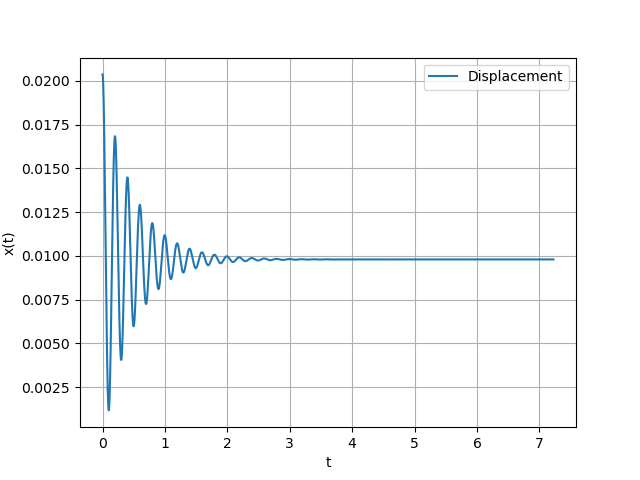
\includegraphics[width=\columnwidth]{figs/fig2.png}
\end{figure}
\end{document}

